\section{Method}

%We first provide the mathematical background for 2D Gaussian Splatting,
%that constitutes the base of our method.
%Starting with our methodology, 
We first define a new representation for appearance of the Gaussian primitives that allows for content-aware texturing.
We then show how to adapt the texturing process to scene content,
by taking into account the different screen-space frequencies that need to be represented using textures.
This is achieved in a progressive manner that is compatible with the optimization process.
Finally,
we propose a resolution-based primitive management method that splits primitives allowing the geometry and appearance of the scene to be approximated as required.


%Throughout our method and depending on the occasion,
In contrast to the original 2D Gaussian Splatting approach~\cite{2dgs} (see
Sec.~\ref{sec:reps} and Eq.~\ref{eq:intersection_point}), we express 
the intersection between a camera ray and a primitive in different coordinate systems, denoted by a superscript.
This is done,
as some coordinate systems make some operations easier.
Specifically:
\begin{itemize}
    \item $\mvec{p}^w = \mvec{p}$ is the intersection point in world space,
    \item $\mvec{p}^{w_0} = \mvec{p}^w - \boldsymbol{\mu}$ is in world space, centered on the primitive,
    \item $\mvec{p}^l = \mvec{R}^{-1}\mvec{p}^{w_0}$ is in the local, axis-aligned coordinate system of the primitive. Since the last component of this point is 0, we consider that $\mvec{p}^l \in \mathbb{R}^2$
    \item $\mvec{p}^{c} = \mvec{S}^{-1}\mvec{p}^l$, where $\mvec{S} = \text{diag}(\boldsymbol{\sigma})$ is in the local, normalised coordinate system of the primitive.
\end{itemize}
This last coordinate system can be considered as the ``canonical'' space of the Gaussian primitive.
The use of these spaces is purely to facilitate some operations.
For instance, \revision{rev9584 typo}{Eq.~\ref{eq:intersection_point}} is evaluated in the camera view space,
where $\mvec{r}_0$ is on top of the origin,
while anything that involves querying the texture map is better done in a coordinate frame local to the respective primitive.

 \revision{rev9584 typo}{The} color of a ray $\mvec{r}$ is computed by alpha blending:
\begin{align}
    \mvec{C(\mvec{r})} &=  \sum_i w_i(\mvec{p}_i)\mvec{c}_i(\mvec{d}) =  \sum_i T_i o_i G_i(\mvec{p}_i)\mvec{c}_i(\mvec{d}) \\
    T_i &= \prod_j^{i-1} (1-o_jG_j(\mvec{p}_j))
\end{align}
where $w_i(\mvec{p}_i)$ is the contribution of the Gaussian, 
$G(\mvec{x})$ is the evaluation of the Gaussian function that defines the falloff $G(\mvec{x}) = e^{-\frac{1}{2}({\mvec{x}^T\mvec{x}})}$, and $T_i$ is transmittance.

% We first define a new representation that allows content-aware texturing for Gaussian Splats. We then show how to adapt the texturing process to scene content, by taking into account the frequencies that need to be represented by texture. This is achieved in a progressive manner that is compatible with the optimization process. Finally, we propose a resolution-based primitive management method that splits primitives to approximate the geometry and appearance of the scene as required.

\subsection{Content-Aware Textures for Gaussian Splats}

%% ADAPT
%In our work, we change the appearance model of 2DGS by including a texture grid for each primitive.  More specifically,
%in addition to the primitive's view-dependent colour,
%we have view-independent texture offsets taken by bilinearly interpolating the values of our grid,
%containing values $\mvec{c}^{\mathbb{T}}$
%So, the primitive colour is now dependent on the intersection point:
%\begin{equation}
%    \mvec{c}(\mvec{p}, \mvec{d}) = \mvec{SH}(\mvec{d}) + \text{B-INTERP}(\mvec{c}^{\mathbb{T}}, u(\mvec{p}), \upsilon(\mvec{p}))
%\end{equation}
%
%\TODO{(Should we explain what we didn't do to proceed to what we did????)} As hinted in the equation above,
%we need a mapping from the intersection point $\mvec{p}$ to the UV coordinates $u$ and $\upsilon$.
%The simplest mapping that we thought of was one from the canonical space of the Gaussian primitive to UV.
%\begin{equation}
%    \mvec{uv} = \frac{\mvec{p}}{2\epsilon} + 0.5
%\end{equation}
%where $\epsilon$ is the extent of the texture in units of standard deviations.



%In this formulation, the texture grid rotates and gets scaled in the same way as the underlying primitive.
%This has the advantage of defining the texture grid with a specific resolution once and then not worrying whether the underlying primitive stretches beyond it, as the grid will rotate and get stretched alongside it.
%Yet, we identified a problem with this definition.  For a constant texture resolution, since the scale of the primitive and that of the texture grid is tied, when the primitive gets scaled up or down during optimisation,
%the individual texels of the texture undergo the same transformation.
%This, however, means that a primitive that grows in size will be able to capture and reconstruct coarser and coarser details.  In a similar manner, a primitive that shrinks in size will see its texture being able to capture finer details, with the risk, however,
%of causing aliasing, when the size of a texel becomes smaller than a pixel.
%\TODO{optimisation????}
%One way to deal with the above issues would be to resample the texture maps to ensure that the texels remain relatively the same size.
%That would still happen in some discrete points in time,
%abruptly affecting the optimisation procedure.
%
%
%\TODO{(Should we explain what we didn't do to proceed to what we did????)} As hinted in the equation above,
%we need a mapping from the intersection point $\mvec{p}$ to the UV coordinates $u$ and $\upsilon$.
%The simplest mapping that we thought of was one from the canonical space of the Gaussian primitive to UV.
%\begin{equation}
%    \mvec{uv} = \frac{\mvec{p}}{2\epsilon} + 0.5
%\end{equation}
%where $\epsilon$ is the extent of the texture in units of standard deviations.
%% REMOVE
%Our method extends 2DGS representation with a texture grid,
%attached in an axis-aligned manner to each primitive.
%In that way,
%we enable multiple colour samples per primitive,
%allowing us to reconstruct high frequency appearance with fewer primitives.
%In the following section we first provide an quick overview of 2DGS and the terminology necessary for our method.
%Then we define the axis-aligned texture grids and how they contribute to spatially varying appearance.
%Finally, we present our strategies for adaptive texel sizes and adaptive density control.

%\begin{itemize}
%\item How to assign and query texture. Basic idea (eq)
%\item Recall that primitives change size during optimization, will cause texture stretching.
%\item As optimization evolves, need to balance between changing texture resolution and adding more primitives. Previous methods either use fixed res BBsplat, Meta; as splitting occurs, resolution gets spread out.
%Alternatively heuristic res adapt based on stretching [Kyros].
%None have principled approach
%\end{itemize}
We augment each 2D Gaussian primitive with a texture map 
%or grid \Fredo{I would drop the term grid. The way it's written is confusing. Is it the same as a texture or an alternative to it?} 
$\mathcal{T}$.
The texture map adds a spatially varying \emph{offset} $\mvec{c}^\mathcal{T}$ to the original spherical harmonic color representation. 
%\Fredo{Why offset?}\TODO{because the take values in [-1,1] range but not explained yet} 
The texture colors vary only spatially and have no directional dependency. This representation is compact and models only the diffuse properties of the surface, akin to albedo multiplied by irradiance. 
%radiance \Fredo{Irradiance I believe because it takes the dot product into account}. 
As a result, the color of each primitive is now also dependent on the intersection point between the ray emanating from the pixel and the 2D primitive:
%In our approach, we augment each 2D Gaussian primitive with a texture grid.
%In addition to the primitive's view-dependent colour,
%we have view-independent texture offsets taken by bilinearly interpolating the values of our grid,
%containing values $\mvec{c}^{\mathbb{T}}$.
%The color of each primitive is now dependent on the intersection point between the ray emanating from the pixel and the 2D primitive:
\begin{equation}
    \mvec{c}_i = \mvec{SH}(\mvec{d}) + \text{bilerp}(\mathcal{T}_i, \mvec{u})
\end{equation}
%Given the intersection point, we need a mapping from the intersection point $\mvec{p}$ to the texel coordinates $u$ and $v$ \TODO{I'd like your opinion on that}\GK{I think it's good, but contrasting it with the previous $c_i(d) = SH_i^{1:b}(d) + SH_i^0$ would make it easier to clarify what we introduced mathematically}.
where $\mvec{u}$ are the coordinates in UV space at which the ray intersects primitive $i$ with a direction vector $\mvec{d}$, and $\mvec{SH}$ are the spherical harmonics.
We need to carefully design the texture coordinate calculation
%texture mapping function 
%\Fredo{Parsing "texture mapping function" was a bit hard for me because texture mapping is the process of using texture. Maybe the texture coordinate function or texture coordinate calculation} 
that transforms the intersection point into local, normalized primitive space $\mvec{p}^c$ to UV coordinates. 
As we discuss below, it is especially important to consider how this mapping changes when the primitive parameters are updated during optimization.
%\Fredo{Say that it's especially important to consider how this mapping changes when the primitive parameters are updated during optimization.}

A simple mapping from the canonical space to UV texture space fixes the relative texture coordinates on the primitive such that the texture will stretch and deform with scaling and rotation of the primitive:
\begin{equation}
\label{eq:basic-u}
    \mvec{u} = \left(\frac{\mvec{p}^c}{2s_i} + 0.5\right)\cdot T_\text{res}
\end{equation}
% where $p$ is the intersection point in local primitive space,
where $s_i$ is the extent of the texture in units of standard deviations of the Gaussian primitive, and $T_\text{res}$ is the texture resolution. When the extent of the texture is smaller than the primitive, some type of padding needs to be applied.

\begin{figure}[!h]
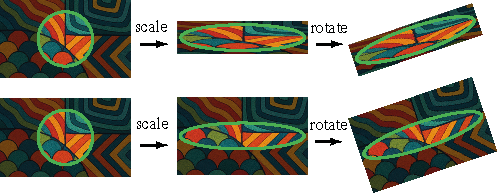
\includegraphics[width=\linewidth]{images/stretch.pdf}
\caption{
\label{fig:stretch}
Difference between two mappings for a primitive having learned a particular texture.
Top row: a naive approach distorts the appearance after the primitive undergoes scaling. Bottom row: in our approach, as texel size is fixed in world space, scaling the primitive only reveals more part of the underlying texture, preserving existing content.
}
\end{figure}
Recall that primitives change size and shape during the optimization process. 
%\Fredo{Avoid long sentences with ";"} 
As a result, with such a texture mapping, the appearance parameters of the texture are coupled with the parameters that control the shape of the primitive. 
During optimization, small changes in the scale of the Gaussians result in changes of all the values of the texture. This can induce local minima in the optimization process that are visible as texture stretching, see Fig.~\ref{fig:stretch} (top).
%to keep appearance the same under small changes in the scale of the Gaussian the optimizer needs to change all the values of the texture. This mapping introduces challenging local minimas in the optimization that manifest as \emph{texture stretching during the optimization.} \TODO{Ideally we would want a toy experiment here to help us with the motivation.}

%\PP{This inherently means that the scale of details that can be represented is tightly tied to the size of the primitives.
%As a primitives grows larger it can represent coarser and coarser details}.
%\PP{To counteract this behavior,
%the only solution is to either dynamically adapt the texture resolution
%or/and add more primitives.}



%as optimization evolves,
%there is a need to balance between adapting texture resolution and adding more primitives.
%Some previous \PP{concurrent, others?} methods use fixed texture resolution ~\cite{bbsplat,textured3dgs};
%\PP{as a result, the only option, the}
%texture resolution/primitive balance is heuristically treated by splitting primitives,
%which results in texture resolution being ``spread out'' across the scene \PP{not sure about this one}.
%Alternatively texture resolution can be adaptively modified based simply on stretching \cite{gstex}.
%These solutions do not take the \emph{content} of the scene in to account, which can result in texture residual stretching and suboptimal distribution of texture resolution.
%\PP{parameter/memory emphasis}
%We illustrate this effect in Fig.~\ref{fig:stretch}(a)-(b).
%\GK{This whole paragraph puzzled me quite a lot: 1) I think "texture resolution" is used very relaxed here, afaik no other related work changes the actual resolution of the texture resolution of the primitives, one can think of adding more primitives increases the "total texture resolution" availiable to the representation but I think the terms are conflated here. 2) I think its dangerous to go through other papers in details in our method because probably reviewers and other readers will not know by heart the literature, and since we have never introduced each other paper in detail it makes the method very hard to read. I would propose to ignore concurrent work until the result section.}
%\TODO{Contrast paragraph with concurrent work, all use (2) we use (3)}
Instead, we define a \emph{content-aware} representation in which textures are adapted to scene content. 
%\Fredo{And discuss positive impact on optimization.}
Our goal is to have textures that can faithfully represent the frequency of image details at the highest resolution present in the input images.
To do this, we fix the texel size with respect to the optimization process such that no optimizable parameters change it. We achieve this with a small modification to Eq.~\ref{eq:basic-u}:
\begin{equation}
    \mvec{u} = \frac{\mvec{p}^l}{k_i} + T_\text{offset}
\end{equation}
\noindent
where $k_i$ is the texel size and $T_\text{offset}$ is an offset to center the texture map.
\revision{rev9584 what does world units mean}{
In constrast to Eq.~\ref{eq:basic-u},
the intersection point $\mvec{p}^l$ and hence the texel size $k_i$ are defined in world space,
with the same units as the primitive's scales $\mvec{\sigma}$.
}

\revision{rev2866 texture resolution unclear}{This mapping implies that the textures do not have a fixed texture resolution.
On the contrary,
as the primitives grow or shrink,
more or less texture resolution is needed to cover their surface.
This is demonstrated in Fig.~\ref{fig:stretch} (bottom).
}
We modified our optimization routines to allocate and de-allocate texture resolution dynamically. %%optimization.

%Changing the scale of a primitive has the sole effect of exposing more or less of same sized texels,
%instead of stretching or contracting them.

Since the number of texels can grow quadratically, we risk running out of resources if every primitive  has a texture. Our goal is to maintain an expressive representation while carefully managing resources. To achieve this, we enforce two properties on our representation: First, the projected sampling frequency of the texture needs to be bounded by the image sampling frequency of the closest camera. This means that the projected texel size should never be smaller than the smallest input pixel that can see it. Second, texel sizes should adapt to \emph{scene content}, i.e., smaller texel sizes should be allocated for high frequency image content.

The first goal can be achieved using a conservative choice to determine minimum texel size as the pixel size back-projected in world space from the input training view closest to the primitive's center $k^p_{\mathrm{min}}$, similarly to \cite{reduced3dgs}.

% \begin{equation}
% \label{eq:kmin}
% {k}^p_{\mathrm{min}} = {w}^p_{\mathrm{min}},
% \end{equation}
% where ${w}^p_{\mathrm{min}}$ is \TODO{PP: complete},
% similarly to the method presented in~\cite{reduced3dgs}. \TODO{PP: say what we do exactly: In practice, we set this value to be 2 times the size of the pixel, which helps avoid aliasing.}

%\PP{I think we should revert to what I've written initially.
%\begin{itemize}
%    \item Introduce the new need of choosing a texel size
%    \item Present our first, 100\% conservative choice
%\end{itemize}
%Our representation/parametrization dictates the selection of a texel size for our primitives.
% Choosing the same texel size for every primitive can pose a problem;
% too big and it can lead to blurry appearance for high-frequency parts of the scene,
% too small and it can cause aliasing for distant views and can be prohibitively memory-intensive.
% So,
% we proceed with the conservative choice,
% which is to use as texel size the pixel size,
% back-projected in world space from the training camera closest to the primitive's center,
% $k = {w}^p_{\mathrm{min}}$,
% similarly to \cite{reduced3dgs}.}

% \PP{
% The choice above ensures that we do not miss any visual detail existing in our training images.
% However,
% the are very few cases
% where the content of the scene is that high frequency
% that a 1-1 correspondance between texels and pixels is needed.
% In contrary,
% in most cases,
% our primitives need to match low frequency content,
% that can be faithfully represented with fewer color samples.
% To allow our primitives to adapt their texture to the frequency content of the input images,
% we extent our texel size by a texel-to-pixel ratio ($t_2p_r$).
% \begin{equation}
%     k = {w}^p_{\mathrm{min}} \cdot \mathrm{t_{2}p}_r
% \end{equation}
% In \cite{gstex, textured3dgs} the texel size is determined at the texture initialisation step,
% and the primitives get assigned a fraction of a total texel budget based on area.
% However,
% this does not take into consideration th
%}

%\PP{we need to discuss this}

%Knowing a-priori the ideal $k_i$ that controls the texel size for each primitive is impractical since primitive scales and distributions dynamically adjust during the optimization. 
Regarding the second goal,
 optimal texel sizes cannot  be determined at initialization
since pritimives change size and rotate dynamically during optimization.
We need a way to adapt to the freqency content of the scene progressively. 
%To that end we introduce during the optimization an adaptive strategy to determine the texel size per primitive. Our method allows to downscale and upscale textures such that regions with high frequency content get allocated textures with smaller texel sizes and low frequency regions coarser textures with larger texel sizes. We build on this observation to propose resolution-aware primitive management.
To do this, we next introduce an adaptive strategy to determine texel size during optimization, where we downscale and upscale texture by adapting to the scene \emph{content}. 
We complement this approach with a resolution-aware primitive management method that add primitives to represent geometric -- rather than appearance -- error.
We describe these two components in the following sections.

%\Fredo{The use of commas "," is often questionable. I have tried to fix it, but be on the lookout. For example, there is usually no comma before that (in contrast to which).}

%We describe the necessary components in the following sections.

% \TODO{I have done until here, took me longer than expected.}
% We could envisage initializing primitive textures by matching resolution from the closest input image. However, we follow standard Gaussian Splatting practice and we initialise our method using the sparse SfM point cloud,  generated during camera calibration. As a result, it would be impractical to initialize all textures using this criterion, since the initial distribution of points (large, non-uniform points etc.) does not provide a sufficient representation of scene geometry. In particular, large points could require very high resolution textures which could be wasteful. 

% Given the need to adapt to frequency content and to progressively achieve resolution matching, 
% we introduce an adaptive strategy to determine texel size during optimization, by introducing a method that allows downscale and upscale of texture. 
% This process provides a set primitives with textures; in regions with large primitives corresponding to high frequency content, required texture resolution will increase. We build on this observation to propose resolution-aware primitive management.
% We describe these two components in the following sections.

% \GK{I think in the last 2-3 paragraphs we are missing an imporant point: We want the texture resolution to be bounded by the matching resolution of the closest image and not necessarily match it since that would be wasteful in cases where the image frequencies are low. }


%%% ADAPT
%In contrary to the above, we chose to define our texture grid on the axis-aligned space, that is, the local coordinates space, in which the axes are scaled by the scales of the primitive, instead of being normalised.  With this formulation the texels have a constant world-space size, independent on the primitive's scale.
%Hence, scaling up or down a primitive has the sole effect of exposing more or less of same sized texels, instead of stretching or contracting a fixed number of them.
%
%This formulation has the advantage of better disentangling the geometry of the primitive, that has to do with its rotation and how big or small it is, from its appearance, as a primitive can grow or shrink without affecting the parts of the scene that it has already fit.
%
%The particularity in this case is that we cannot set the texture resolution, as it changes dynamically with the size of the primitive.  Instead, we need to set the texel size for each primitive.  To avoid choosing a fixed size for all primitives, something that could prove to be too wasteful and aliasing inducing or too coarse and inappropriate,
%depending on the how small or big it would be, we decided to be conservative and choose as texel size the world size width of a pixel, back projected to the centers of our primitives, taken by the closest training camera.  That ensures that on one hand, primitives have the capacity to reconstruct the finest observable details and on the other hand, primitives that are consistently observed from afar do not have too small texels, causing aliasing and wasting memory.
%
%\TODO{that's tricky to explain because it's a bit of an implementation issue. the UV coordinates need some texture resolution to be constrained in the 0-1 range and I think that'll more confusing than just saying, we query our texture like that} The mapping in this case goes directly to the texture indices,
%



%\begin{itemize}
%\item Instead we define a content-aware texture representation in which world-space texel size is adapted to represent the content in the input images.
%\item Diagram showing cases
%\item In practice, texel size needs to be adapted during optimization. We next explain the steps of our method.
%\end{itemize}

\subsection{Progressive Adaptive Texel Size Determination}

%\begin{itemize}
%\item Then we need to do this adaptively Notion of texture detail, requirement of frequency
%\item Have an additional parameter that allows finer control $t2p_r$, adapt to frequency
%\item Then downscale upscale definition
%\item Progressive algorithm: start with 2DGS (500 iterations), warm up wo textures. Then init everyone to 8x8 and compute $t2p_r$, for the next few hundreds of iterations, downscale and upscale will find resolution that is adapted to content.
%\item We next talk about splitting
%\end{itemize}

%The choice of texel size made above is, as already mentioned, conservative to the finest observable detail.
%However, in most cases, primitives do not need that high of a granularity, as they might be in parts of the scene with coarse details.
%In these cases, having approximately one texel per pixel is too wasteful in terms of memory and may also cause optimisation issues due to overparametrisation.

Our goal is to adapt textures to the frequency content of the input images. We also need to achieve this in a progressive manner that fits well with the optimization process. We define a \emph{texel size-to-pixel} size ratio ${t_{2}p}_r$, which we manipulate during optimization using downscaling and upscaling operations.

We define the texel size $k$ based on the minimum pixel size ${k}^p_{\mathrm{min}}$, with ${t_{2}p}_r$ as follows:
\begin{equation}
    k = {k}^p_{\mathrm{min}} \cdot {t_{2}p}_r
\end{equation}

\noindent
%This reparametrisation offers us a knob 
%that we can use to adjust the size of the texels of individual primitives,
%depending on the underlying content of the scene. \TODO{giving us more control on parameter/memory budget}.
We use this parameter to assign a low $t_2p_r$ to primitives in regions with fine details.
% \GK{I don't understand that, let's say you have 1:1 texel to pixel ratio, this means you have one texel to pixel that bounds the frequency of the images, an even lower texel to pixel ratio i.e 1:10 mean you have one texel for 10 pixels - are we sure low here is what we want?}
As a result, such primitives will have more texels for a given primitive size.
Similarly, primitives that lie in areas with low-frequency appearance will have a higher ratio,
giving them relatively fewer texels.
% \GK{do we bound texel-to-pixel ratio  between (0,1]? if we do this is the section to mention it.}
To provide a lower bound of 1 and facilitate texture rescaling operations,
$t_2p_r$ can only take values that are powers of two.

To this end, we propose two strategies to increase and decrease $t_2p_r$
leading to a downscale and an upscale of the texture map respectively.
Note that texel size and texture resolution are linked, but not the same. In the operations below, when texel size changes, texture resolution will change but only because the \emph{primitive size is unchanged}.

\begin{figure}[!h]
	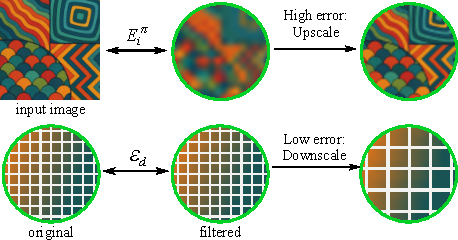
\includegraphics[width=\linewidth]{images/upscale_downscale/updownscale.pdf}
\caption{
\label{fig:down-up}
We illustrate the downscale and upscale process used.
}
\end{figure}

\textbf{Increase of texel size-to-pixel size ratio - Downscaling}:
Our goal is to find texture maps that represent low frequency details and decrease their texel size accordingly.
We do this by applying a low-pass filter on textures and then comparing them to the originals.
The error $\mathcal{E}_d$ is weighted by the Gaussian falloff of the primitive,
leading to the following equation:
\begin{equation}
    \mathcal{E}_d = \frac{1}{\sum_\mvec{p}G(\mvec{p})}\sum_\mvec{p}G(\mvec{p})(T_\mathrm{orig}(\mvec{p}) - T_\mathrm{lowpass}(\mvec{p}))
\end{equation}

If this error is less than a threshold $\tau_\text{ds}$,
we assume that the texture map can be reconstructed with good-enough fidelity by the downscaled version.
Hence, we double  ${t_{2}p}_r$, which
reduces the total number of texture parameters by 4.
This reduces the resolution of texture, since the world-space size of the texels has grown. The size of the primitive is however unchanged. 

\textbf{Decrease of texel size-to-pixel size ratio - Upscaling}:
In regions where the texel size of the primitives involved is too large to capture the fine, underlying details, we expect our images to be blurry, and thus induce large error.
To identify these regions, we estimate primitive error using the approach presented in~\cite{revising}.
Specifically, for a primitive $i$, a ray $\mvec{r}$, a camera view $\pi$ and corresponding RGB error image $\mathcal{E}_\pi$,
we compute the per primitive error for a single view:
\begin{equation}
    E^\pi_i = \sum_{\mvec{r} \in \mathcal{P}_i} \mathcal{E}_\pi(\mvec{r})w^\pi_i(\mvec{r})
\end{equation}
where $\mathcal{P}_i$ are all the pixels covered by the primitive.
%TODO{In a slight abuse of notation,
Here we assume that we have one ray per pixel,
emanating from its center.
Differently from \cite{revising},
instead of taking the maximum error over views, %aggregating the errors across images with a max operator,
we perform a weighted sum,
with the weight being the total contribution of a primitive in that image.
\begin{equation}
    E_i = \frac{\sum_{\mvec{\pi} \in \Pi} E^\pi_i \overline{w_i^\pi}}{\sum_{\mvec{\pi} \in \Pi} \overline{w_i^\pi}}, \quad
    \overline{w_i^\pi} = \sum_{\mvec{r} \in \mathcal{P}_i}w_i^\pi(\mvec{r})
\end{equation}

\noindent
where $\Pi$ is the set of all input views.
%Concisely,
This choice assigns an error value to each primitive that is proportional to their contribution to the rendered image.

We choose the top 10\% of primitives with the highest error, and upscale their textures by a factor of 4,
by halving $t_2p_r$.
With smaller sized texels,
these primitives can better fit to the scene content,
reducing their error.

\textbf{Progressive texel size adaptation.}
The calculation of the per primitive error $E_i$ and
the application of upscale/downscale process happens regularly during optimization.
Texel size adapts to scene content during this process, getting bigger for primitives that lie in low-frequency regions, and smaller for primitives that exhibit large error,
as shown in Fig.~\ref{fig:teaser}(right).
%Specifically for the latter case,
%it is expected that the error associated with a primitive drops as it gets upscaled,
%as more and finer texels are assigned to it and thus it can better fit the content.
%However,
%this is not always the case,
%because the error can appear in regions that are badly reconstructed,
%in terms of geometry i.e. missing objects.

There are two main sources of error: appearance and geometry. For the first case, our upscaling approach reduces error as the optimization progresses.
However, for the case of geometry that is not well represented, an additional step is required.
% To initialize the process,
% we run 500 iterations of 2DGS where each primitive has a single constant color.
% At this point,
% we assign an 8x8 texture to all primitives \PP{we set the $t_2p_r$ of our primitives so that their smallest dimension has 8 texels}, then continue optimization,
% calculating the error and applying the upscale/downscale process every 250 iterations.
% Consequently,
% after a few of these steps,
% some primitives will have high-resolution textures,
% corresponding to regions with fine detail.
% In such cases,
% such primitives often need to be split,
% either to better capture \emph{geometry detail} or to strike a better balance between memory used for primitive parameters and texture offsets.
To address this and complete our content-aware method, we next introduce resolution-aware splitting.

% \begin{itemize}
%     \item The ratio 1 pixel per texel is too wasteful on memory. So let's have multiples of the base
%     \item So we need a way to change the size of texels. We parametrize the texel size as minimum\_pixel\_width * pixel\_texel ratio, where that latter is a power of 2
%     \item Choosing a global texel size is challenging, since 1) not every area has the same scale of details and being conservative is wasteful
%     \item We develop 2 strategies to change this value.
%     \item Increase the texel size (downscale): Downscale our textures by a factor of 2 using bicubic interpolation. Upscale using bicubic interpolation. Compare the reconstructed and the original with an L1 loss * the opacity and the falloff (alpha value). If that loss is small, lower than a threshold, then we assume that the texture is simple enough so the downscaled version can be used. This reduces the memory for a particular texture by a factor of 4!
%     \item Decrease the texel size (upscale): As this has an effect on memory, we want to do it only in regions where it's needed. And what's a better criterion than the actual error we optimise for??? So we compute this error from all views, weighted by the primitives' contributions. We then pick the 10\% of primitives with the highest error and we upscale them by a factor of 2, using nearest neighbour interpolation, to have zero-effect on the scene. This increases the memory of a particular texture by a factor of 4.
%     We set set the minimum pixel\_texel\_ratio to 2, because we noticed that blending allows to get details of subtexel scale, by combining colours from multiple primitives, so we don't lose any expressivity.
% \end{itemize}
    
\subsection{Resolution-aware Primitive Management}
% \PP{Need to discuss this
% I like the 3 paragraphs.
% However, I prefer the layout I had made,
% 1)"Adaptive texel size to match appearance" (previous section)
% 2)"Densification to add points" (the standard SfM is too sparse and not even our super points can deal with that sparseness + flat planes approximation; no one will tell us off because we didn't give a better intuition on why we need densification, not even original 3dgs explained in-depth why.)
% 3)Since our error is RGB, we use texture resolution as threshold (these 3 paragraphs),
% implying that if we had both RGB and geometric error this wouldn't be necessary (never tested, unfortunately, but is very probably true).
% On the other hand I can get that this might be too complicated.
% }

%Even with our more expressive points,
%this point cloud is too sparse,
%so we also need to employ Adaptive Density Control (ADC)
%to add points in parts of the scene that are not well reconstructed.
%Because our primitives are more expressive and carry more parameters with them,
%cloning strategies used by the original method and others
%\cite{Kerbl_2023}
%\missingcitation{MCMC, 3dgs, revising},
%that work by stacking points on top of each other
%are not appropriate.
%Instead,
%we opted for a splitting strategy, similar to the \missingcitation{revising densification} one.
%
%In the same way as in the upscaling strategy,
%for the 10\% primitives with the highest error
%we check which of those exceed a size threshold.
%These primitives get replaced by two primitives,
%displaced by +- 1 size (std),
%having half the respective scale
%and $G(1)$ the opacity.
%
%The texture grids of the newly added points results from the original one by sampling it at the respective locations.
%
% \begin{itemize}
%     \item The initial point cloud is too sparse. We need a way to add points.
%     \item The original cloning method or other methods that are based on cloning like MCMC \missingcitation{mcmc} have the undesireable effect of stacking a lot of points on top of each other. As our primitives are heavier in terms of parameters and in general, can overfit more easily, such a strategy proved to be unsuitable, both in terms of memory and quality
%     \item However, with our new primitives we can construct a better splitting strategy. Let's define the properties that we want to have.
%     1) Primitives that well reconstruct their part of the scene should remain untouched
%     2) Primitives that reconstruct their part of the scene badly should be spilt into smaller primitives that add more degrees of freedom in terms of geometry, and hence are more flexible.
%     3) To avoid adding too many primitives and flocking the optimiser with parameters, we want to apply that to primitives that have a size greater than a threshold
%     \item So primitives above a size and error threshold get split into two, along the overflowing dimension.
% \end{itemize}

%The choice of this size threshold is discussed in the next section.

%\subsection{Source of errors and Interplay}

% During optimisation, we don't know why a primitive has error.
% There are 2 cases.
% 1) the primitive has the correct appearance, but doesn't match the geometry. Since we have flat primitives, that means that they might protrude/poke out from some views. In this case we need more fine-grained geometry, which can be achieved by getting more points
% 2) the primitive matches the surface but doesn't match the appearance. This case didn't exist in the original method since the number of colour and geometric samples was tied. In our case, though, we can deal that by increasing the colour samples, something that can be done by reducing the texel\_pixel\_ratio
%\TODO{maybe put it in the beginning, as a discussion, in a more "general" way. Like, let's say we have primitives that can match the appearance and geometry separately, describe what we want, and then proceed into the two methods that actually do this}



In Gaussian splatting methods where each primitive contains one color sample, \emph{densification} -- i.e., adding new primitives through cloning and splitting -- plays an essential role in improving the reconstruction of the scene.
This results in a local increase in both the geometric (position, scale, rotation) and appearance parameters (SH, opacity) that are treated together since they are tied to a single Gaussian primitive. 
%hence increasing, locally,
%both the geometric and the appearance degrees of freedom/parameters.
However, this is not always ideal, since there are cases where the geometry is low frequency and has been approximated well, but we are missing texture detail, or conversely, cases where the color information is low frequency, but the underlying surface is not correctly represented. The latter case can appears as holes, ``softened'' edges or elongated primitives in places where they are not required. 

\begin{figure}[!h]
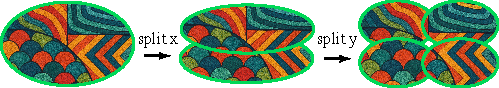
\includegraphics[width=\linewidth]{images/split.pdf} 
\caption{
\label{fig:splitting}
Left to right:The primitive has been upscaled to a resolution greater than $\tau_{tr}$ in both axes. Our splitting approach creates four new primitives, each with half the scale and texture resolution in both axes.}
\end{figure}


Our separation of geometric and appearance parameters provides an additional degree of freedom, allowing us to independently decide whether to increase the number of parameters linked to \emph{geometry}, i.e., increasing the number of primitives or to \emph{appearance}, i.e., increasing texture resolution.

Given that we do not have a supervision signal explicitly for geometry, 
%In our framework,
%we can use the two strategies introduced in sections and 
%to essentially inject geometric and appearance parameters \textbf{separately} to our scenes,
%to address these two sources of error.
%For the first one we can upscale the respective primitives to add more colour samples,
%while for the second one,
%we can split the existing primitives to add more geometric degrees of freedom.
%However,
%since our representation is supervised by the appearance (we don't use any geometric supervision),
we attempt to first match the appearance, using the upscaling approach described above.
If the error is still high despite upscaling,
we interpret the remaining error as geometric.
In these cases,
we can add more primitives,
locally increasing the geometric degrees of freedom.
\revision{rev2866 3dgs-mcmc}{
We found that densification strategies that were based on cloning either partially \cite{3dgs} or entirely in the case of 3DGS-MCMC \cite{3dgs-mcmc}, are incompatible with our representation. This is because
the superimposition of multiple textured primitives makes convergence difficult and requires an excessive number of parameters.
As a result our primitive management is based on \emph{splitting}, which fits well with our method. We describe this next.
%that is adjusted to the rest of the framework and is described next.
}

%And that is done by taking the texture resolution as the size threshold.

Similar to the approach for upscaling, we take the top 10\% of primitives with the highest error, and check which of these exceed a threshold $\tau_{\mathrm{tr}}$ for texture resolution. The primitive is replaced by two new primitives, each displaced by $\pm 1$ standard deviation of the Gaussian.
This process is performed separately for each axis; the new primitives have half the scale (size) in each corresponding axis,
as a result, half the texture resolution,
$G(1)$ times the opacity, where $G$ is the Gaussian.
The texture map of the newly added primitives is created by sampling the original point at the respective locations.
Fig.~\ref{fig:splitting} illustrates the splitting process for a primitive that happens to have a texture resolution greater than $\tau_{\mathrm{tr}}$ in both axes. A flowchart of how upscaling and splitting interact is shown in Fig.~\ref{fig:densify}. Alg.~\ref{alg:routines} displays in high level how the two methods are integrated in code.

\begin{figure}[!h]
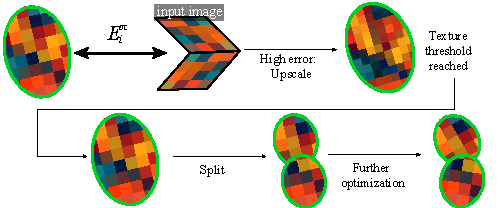
\includegraphics[width=\linewidth]{images/densify/densify.pdf} 
\caption{
\label{fig:densify}
The primitive has high error, and successive upscalings result in a texture resolution above threshold. In this case, the error is geometric rather than due to appearance. Our algorithm performs a split, and further optimization will match the geometry.}
\end{figure}


% With the upscaling strategy described above,
% our primitives can acquire complex appearances to match the underlying scene content.
% For that to happen though,
% it is imperative that the primitives approximate the underlying geometry well,
% because otherwise multi-view inconsistencies can hinder or even entirely prevent the learning of one, consistent appearance.
% As our primitives are flat,
% they can only provide a planar approximation of the surfaces,
% the granularity \TODO{find a better word?} of which depends on the primitives' sizes.
% However,
% in cases where the primitive density is low,
% either due to the initialisation or the optimisation procedure,
% and does not allow the primitives to become small (as there would be holes otherwise),
% we need a way to add new points,
% that is compatible to our representation.
% More specifically,
% since our primitives are more expressive and carry more parameters with them,
% cloning strategies used by the original method and others \missingcitation{MCMC, 3dgs, revising},
% that work by stacking points on top of each other
% are note appropriate.


% Since this complicates both strategies of adaptive texel size and adding new points,
% we decided to create a link between the two,
% to create an interplay.
% This link is choosing the size of the splitting criterion to be the texture resolution of a primitive.

% In that way,
% a primitive without error is left unaltered.
% If a primitive has error,
% this strategy will first try to correct that by assigning more colour samples to it, increasing its resolution.
% If this gets too high, then the primitive will be split into multiple primitives,
% each one having a fraction of the original resolution.
% These smaller primitives can attach themselves better to surfaces,
% and since they represent more localised appearance,
% they can have simpler textures,
% enabling downscaling.


\begin{table*}[!ht]
\footnotesize
\setlength\tabcolsep{1.5pt}
\centering
\scalebox{0.85}{
\begin{tabular}{@{}>{\raggedright\arraybackslash}p{1.8cm}|>{\centering\arraybackslash}p{0.8cm}>{\centering\arraybackslash}p{0.8cm}>{\centering\arraybackslash}p{0.8cm}>{\centering\arraybackslash}p{0.8cm}>{\raggedleft\arraybackslash}p{0.8cm}>{\centering\arraybackslash}p{0.9cm}>{\centering\arraybackslash}p{0.55cm}|>{\centering\arraybackslash}p{0.8cm}>{\centering\arraybackslash}p{0.8cm}>{\centering\arraybackslash}p{0.8cm}>{\centering\arraybackslash}p{0.8cm}>{\raggedleft\arraybackslash}p{0.8cm}>{\centering\arraybackslash}p{0.9cm}>{\centering\arraybackslash}p{0.55cm}|>{\centering\arraybackslash}p{0.8cm}>{\centering\arraybackslash}p{0.8cm}>{\centering\arraybackslash}p{0.8cm}>{\centering\arraybackslash}p{0.8cm}>{\raggedleft\arraybackslash}p{0.8cm}>{\centering\arraybackslash}p{0.9cm}>{\centering\arraybackslash}p{0.55cm}}
 & \multicolumn{7}{c|}{DeepBlending} & \multicolumn{7}{c|}{Mip-Nerf-360} & \multicolumn{7}{c}{Tanks\&Temples} \\
 & SSIM$\uparrow$ & PSNR$\uparrow$ & LPIPS$\downarrow$ & Points & Texels & Params & FPS & SSIM$\uparrow$ & PSNR$\uparrow$ & LPIPS$\downarrow$ & Points & Texels & Params & FPS & SSIM$\uparrow$ & PSNR$\uparrow$ & LPIPS$\downarrow$ & Points & Texels & Params & FPS \\
\midrule
3DGS-MCMC &  0.903 & 29.81 & 0.311 & 1323K & 0.0M & 78.1M & 265 & 0.831 & 27.82 & 0.232 & 2587K & 0.0M & 152.6M & 103 & 0.855 & 24.25 & 0.211 & 695K & 0.0M & 41.1M & 230 \\
\midrule
2DGS* & {\cellcolor{tabthird}} 0.899 & {\cellcolor{tabthird}} 29.52 & 0.324 & 1444K & 0.0M & {\cellcolor{tabsecond}} 83.8M & {\cellcolor{tabfirst}} 96 & {\cellcolor{tabsecond}} 0.801 & {\cellcolor{tabfirst}} 27.18 & {\cellcolor{tabthird}} 0.282 & 2079K & 0.0M & {\cellcolor{tabfirst}} 120.6M & {\cellcolor{tabfirst}} 91 & 0.834 & 23.37 & {\cellcolor{tabthird}} 0.239 & 872K & 0.0M & {\cellcolor{tabsecond}} 50.6M & {\cellcolor{tabfirst}} 165 \\
BBSplat & 0.898 & 29.25 & {\cellcolor{tabsecond}} 0.318 & 160K & 41.0M & 173.0M & {\cellcolor{tabthird}} 27 & 0.781 & 26.67 & {\cellcolor{tabsecond}} 0.273 & 237K & 60.9M & 257.0M & {\cellcolor{tabthird}} 23 & {\cellcolor{tabfirst}} 0.848 & {\cellcolor{tabfirst}} 23.62 & {\cellcolor{tabfirst}} 0.178 & 300K & 76.8M & 324.3M & {\cellcolor{tabthird}} 38 \\
GSTex & {\cellcolor{tabsecond}} 0.906 & {\cellcolor{tabsecond}} 29.63 & {\cellcolor{tabthird}} 0.323 & 1503K & 10.0M & {\cellcolor{tabthird}} 117.2M & 21 & {\cellcolor{tabfirst}} 0.802 & {\cellcolor{tabsecond}} 27.06 & 0.285 & 2025K & 10.0M & {\cellcolor{tabsecond}} 147.5M & 20 & {\cellcolor{tabsecond}} 0.842 & {\cellcolor{tabsecond}} 23.48 & 0.240 & 877K & 10.0M & {\cellcolor{tabthird}} 80.9M & 20 \\
Ours & {\cellcolor{tabfirst}} 0.907 & {\cellcolor{tabfirst}} 30.03 & {\cellcolor{tabfirst}} 0.303 & 222K & 21.6M & {\cellcolor{tabfirst}} 78.1M & {\cellcolor{tabsecond}} 70 & {\cellcolor{tabthird}} 0.795 & {\cellcolor{tabthird}} 27.00 & {\cellcolor{tabfirst}} 0.263 & 218K & 46.6M & {\cellcolor{tabthird}} 152.6M & {\cellcolor{tabsecond}} 67 & {\cellcolor{tabthird}} 0.835 & {\cellcolor{tabthird}} 23.43 & {\cellcolor{tabsecond}} 0.225 & 164K & 10.4M & {\cellcolor{tabfirst}} 41.1M & {\cellcolor{tabsecond}} 121 \\
\end{tabular}
}

\caption{\label{tab:default-eval}
We compare our method against 2DGS* trained with no geometric regularisations,
BBSplat and GSTex, with default settings.
We show standard quality metrics (PSNR, SSIM, L-PIPS), total number of primitives, texels and parameters.
Our method achieves competitive results while using significantly fewer, highly expressive primitives. \revision{}{We also include 3DGS-MCMC for completeness; please note that 3DGS-based methods achieve better NVS but worse geometry quality compared to all approaches based on 2DGS (see discussion Sec.~\ref{sec:eval}).} }

\end{table*}

\begin{table*}[!ht]
\footnotesize
\setlength\tabcolsep{2pt}
\centering
\scalebox{0.85}{
\begin{tabular}{@{}>{\raggedright\arraybackslash}p{1.1cm}|>{\centering\arraybackslash}p{0.8cm}>{\centering\arraybackslash}p{0.8cm}>{\centering\arraybackslash}p{0.8cm}>{\centering\arraybackslash}p{0.8cm}>{\raggedleft\arraybackslash}p{0.8cm}>{\centering\arraybackslash}p{0.9cm}>{\centering\arraybackslash}p{0.55cm}|>{\centering\arraybackslash}p{0.8cm}>{\centering\arraybackslash}p{0.8cm}>{\centering\arraybackslash}p{0.8cm}>{\centering\arraybackslash}p{0.8cm}>{\raggedleft\arraybackslash}p{0.8cm}>{\centering\arraybackslash}p{0.9cm}>{\centering\arraybackslash}p{0.55cm}|>{\centering\arraybackslash}p{0.8cm}>{\centering\arraybackslash}p{0.8cm}>{\centering\arraybackslash}p{0.8cm}>{\centering\arraybackslash}p{0.8cm}>{\raggedleft\arraybackslash}p{0.8cm}>{\centering\arraybackslash}p{0.9cm}>{\centering\arraybackslash}p{0.55cm}}
 & \multicolumn{7}{c|}{DeepBlending} & \multicolumn{7}{c|}{Mip-Nerf-360} & \multicolumn{7}{c}{Tanks\&Temples} \\
 & SSIM$\uparrow$ & PSNR$\uparrow$ & LPIPS$\downarrow$ & Points & Texels & Params & FPS & SSIM$\uparrow$ & PSNR$\uparrow$ & LPIPS$\downarrow$ & Points & Texels & Params & FPS & SSIM$\uparrow$ & PSNR$\uparrow$ & LPIPS$\downarrow$ & Points & Texels & Params & FPS \\
\midrule
BBSplat & {\cellcolor{tabthird}} 0.895 & {\cellcolor{tabsecond}} 28.93 & {\cellcolor{tabsecond}} 0.332 & 72K & 18.5M & 78.1M & {\cellcolor{tabthird}} 57 & {\cellcolor{tabsecond}} 0.768 & {\cellcolor{tabsecond}} 26.02 & {\cellcolor{tabsecond}} 0.291 & 141K & 36.1M & 152.6M & {\cellcolor{tabthird}} 33 & {\cellcolor{tabsecond}} 0.801 & {\cellcolor{tabsecond}} 22.77 & {\cellcolor{tabsecond}} 0.259 & 47K & 12.3M & 51.8M & {\cellcolor{tabsecond}} 87 \\
GSTex & {\cellcolor{tabsecond}} 0.896 & {\cellcolor{tabthird}} 28.29 & {\cellcolor{tabthird}} 0.354 & 222K & 21.6M & 78.1M & {\cellcolor{tabsecond}} 60 & {\cellcolor{tabthird}} 0.748 & {\cellcolor{tabthird}} 25.19 & {\cellcolor{tabthird}} 0.352 & 217K & 46.6M & 152.6M & {\cellcolor{tabsecond}} 46 & {\cellcolor{tabthird}} 0.745 & {\cellcolor{tabthird}} 20.65 & {\cellcolor{tabthird}} 0.363 & 164K & 10.4M & 41.1M & {\cellcolor{tabthird}} 67 \\
Ours & {\cellcolor{tabfirst}} 0.907 & {\cellcolor{tabfirst}} 30.03 & {\cellcolor{tabfirst}} 0.303 & 222K & 21.6M & 78.1M & {\cellcolor{tabfirst}} 70 & {\cellcolor{tabfirst}} 0.795 & {\cellcolor{tabfirst}} 27.00 & {\cellcolor{tabfirst}} 0.263 & 218K & 46.6M & 152.6M & {\cellcolor{tabfirst}} 67 & {\cellcolor{tabfirst}} 0.835 & {\cellcolor{tabfirst}} 23.43 & {\cellcolor{tabfirst}} 0.225 & 164K & 10.4M & 41.1M & {\cellcolor{tabfirst}} 121 \\
\end{tabular}
}


\caption{\label{tab:same-param-eval}
We compare against BBSplat and GSTex in a same parameter setting,
by adjusting their primitive count and texels accordingly.
The slight discrepancy in BBSplat's parameters in Tanks \& Temples is due to a sphere sampling method they use to model the background and distant objects.
}
\end{table*}


\subsection{Training and Regularisation}
As in \cite{3dgs},
we train our model using the weighted sum of the per-pixel $\mathcal{L}_1$
and the structural similarity losses,
between the ground truth and the rendered images:
\begin{equation}
    \mathcal{L}_{\text{RGB}} = (1-\lambda_{\text{SSIM}})\mathcal{L}_1 + \lambda_{\text{SSIM}}\mathcal{L}_{\text{SSIM}}
\end{equation}
with $\lambda_{\text{SSIM}}=0.2$.

We observed that textures could finish converging to high-frequency settings,
even though alpha-blending would create a smooth result.
This prevented them from being downscaled,
leading to high parameter usage.
To resolve this,
we apply a sparsity regularization on the texel values,
pushing them towards zero,
\begin{equation}
    \mathcal{L}_{\text{texture}} = \lambda_{\text{texture}} \sum_i |\mvec{c}_i^{\mathcal{T}_i}|
\end{equation}
We constrain the texel values in the $[-1,1]$ range,
using a sigmoid activation,
scaled and shifted accordingly:
\begin{equation}
    \mvec{c}^{\mathcal{T}_i} = 2\sigma(\mvec{c}'^{\mathcal{T}_i})-1
\end{equation}
where $\sigma(x)$ is the sigmoid function and $\mvec{c}'^{\mathcal{T}_i}$ are the unactivated texture features.
Intuitively,
this parametrization coupled with the sparsity loss
forces the view-dependent color $\mvec{SH}(\mvec{d})$ to learn the base color of the surface,
while the texels operate as offsets to model high-frequency details.
An example of this is illustrated in Fig.~\ref{fig:teaser}(left).

Finally,
as in \cite{reduced3dgs, 3dgs-mcmc},
we incentivize low-contribution primitives to effectively disappear by applying an opacity regularization term:
\begin{equation}
    \mathcal{L}_{\text{opacity}} = \lambda_{\text{opacity}} \frac{1}{N}\sum_i^N \mvec{o}_i.
\end{equation}

Taking both training objectives and regularizations into consideration,
the total loss is formed as:
\begin{equation}
    \mathcal{L} = \mathcal{L}_{\text{RGB}} + \mathcal{L}_{\text{texture}} + \mathcal{L}_{\text{opacity}}.
\end{equation}
